\documentclass[UTF8]{ctexart}

\usepackage{subfiles}  

%下面的语句, 引入你的头部设置文件
\usepackage{C:/phpStorm_proj/02_myself_ID_EGO/+100_latex_all_math_sel/myPreamble} 
%必须是绝对路径,才能让各个tex在单独编译时使用到

\title{行列式}


%---------------------------------


\begin{document}
	\tableofcontents % 生成目录
	\date{} % 若不写这句, 则默认也会渲染出日期, 所以我们要手动赋空值
	\maketitle  %这行代码, 让你前面的 title, author, date生效
	
	
	
	
	\section{二阶与三阶行列式}
	
	\subsection{二阶行列式}
	
	$
	\left| \begin{matrix}
		a&		b\\
		c&		d\\
	\end{matrix} \right|=\underset{\text{主对角线}}{\underbrace{ad}}-\underset{\text{副对角线}}{\underbrace{bc}}
	$
	
	
	
		\subsection{三阶行列式}
	$
	\left| \begin{matrix}
		a&		b&		c\\
		d&		e&		f\\
		h&		i&		j\\
	\end{matrix} \right|=\left( aej+bfh+cdi \right) -\left( ceh+dbj+aif \right) 
	$ \\
	
	即: \\
	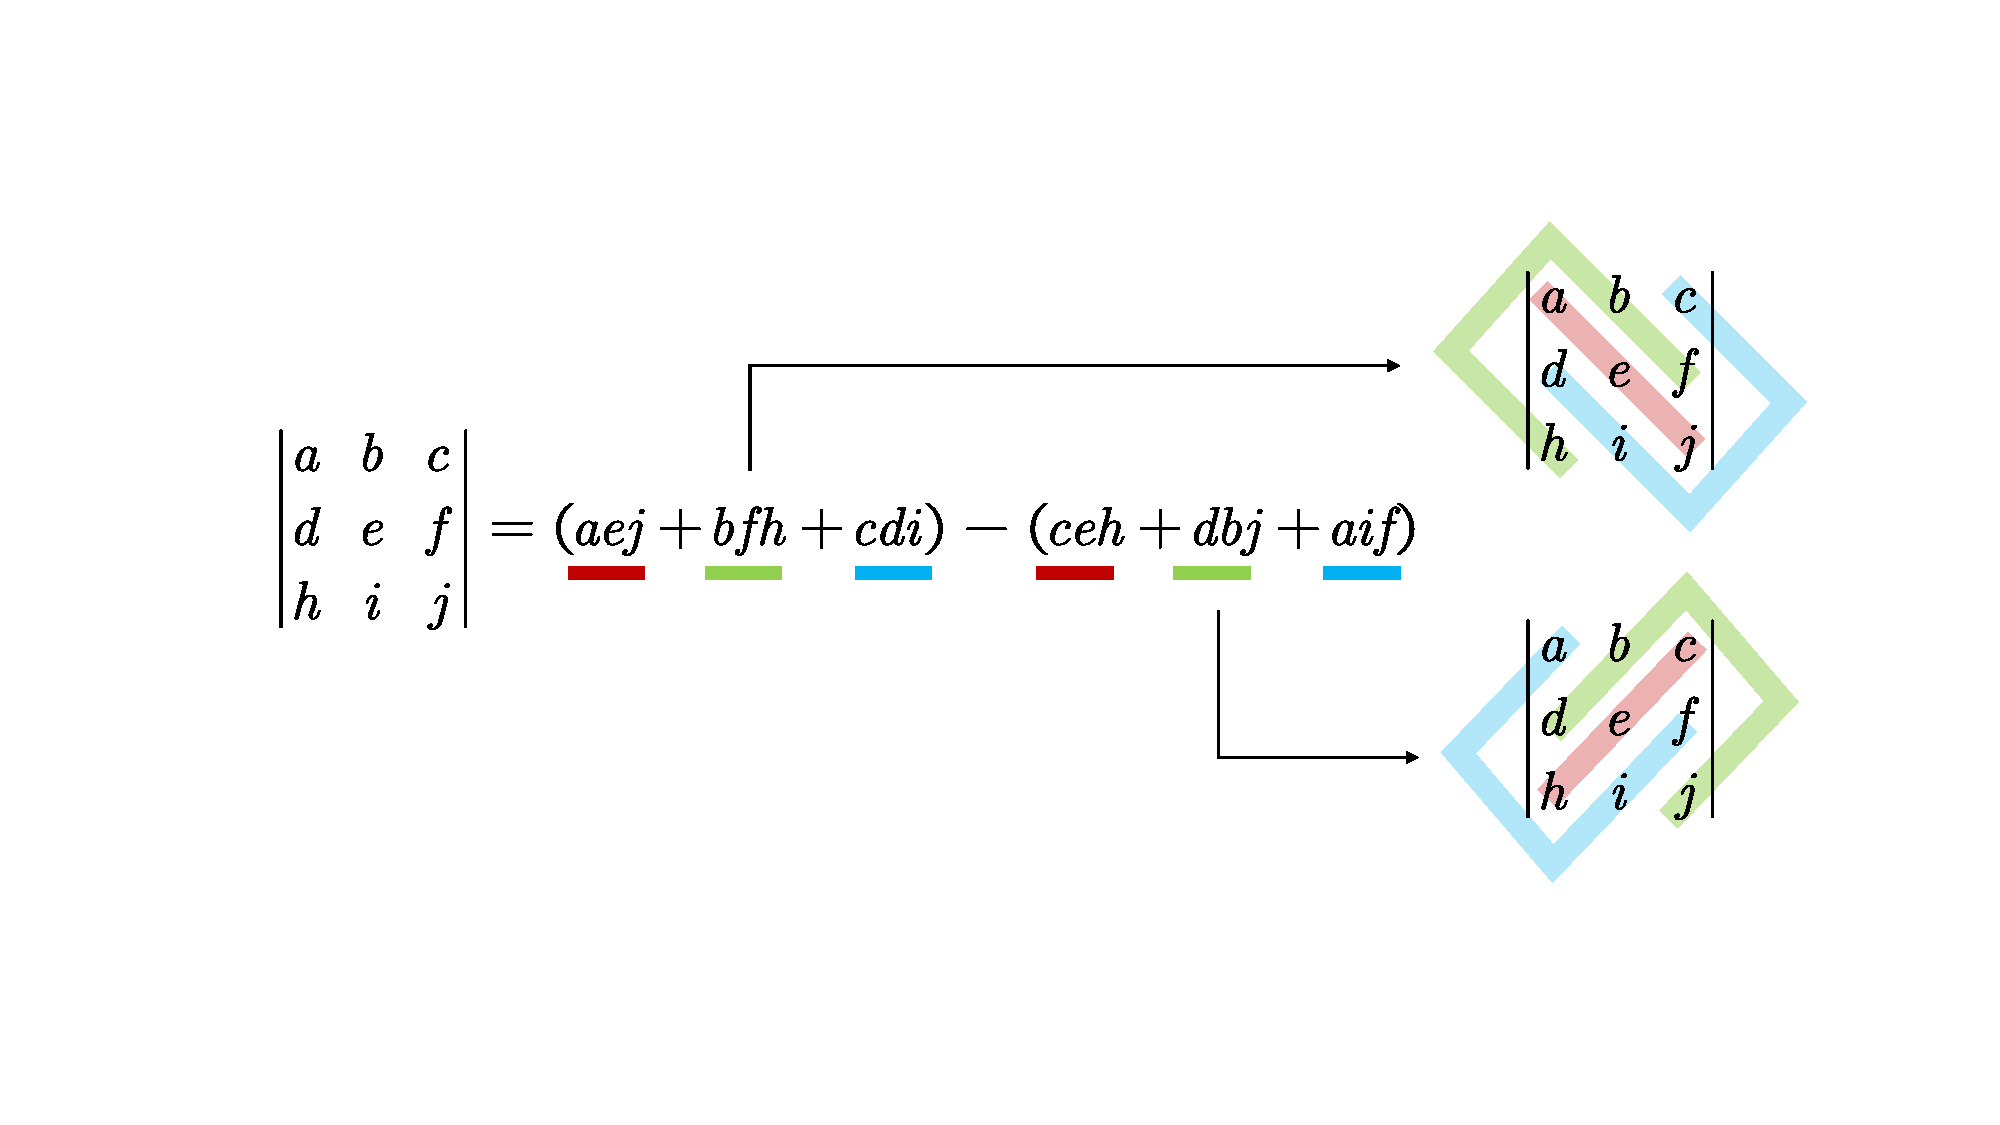
\includegraphics[width=0.8\textwidth]{img/0001.pdf}\\
	
	
	
	
	\section{全排列和对换}
	
	【排列】:\\
	由1,2,...,n 组成的一个``有序"数组, 叫``n级排列".\\
	注意: (1)它是有"顺序"的. 比如: \textbf{1}23, 132, \textbf{2}13, 231, \textbf{3}12, 321.  ← 这个就叫``3级排列".\\
	
	(2)它中间不能缺数, 必须是包含1,2,3...到n的 全部这n个数字, 中间不能缺少任何一个数字. \\
	那么n个数字, 它的全排列(就是排列组合中的排列), 有多少种可能性呢? 那就是: 第1个数字的位置上, 可以从这种n个数字中任取一个出来放. 第二个位置上, 就是从 n-1 的数字中,任取一个出来摆放..., 一共就有: $n\cdot \left( n-1 \right) \cdot \left( n-2 \right) \cdot ...\cdot 3\cdot 2\cdot 1 = n!	$ 种排列方式.\\
	
	
	【逆序】:\\
	``大的数字"排在``小的数字"的前面, 就叫``逆序". 比如: 4213,  4这个大数字, 排在了2这个小数字的前面. \\
	
	
	【逆序数 negative】:\\	
	就是逆序的总数, 你只要数一数有多少个``逆序"存在, 这个总数就是``逆序数".\\
	比如, 4213, 它的逆序有: \\
	- 4后面, 有3个数字比它小 (即2, 1, 3) \\
	- 2后面, 有一个比它小 (即数字1). \\
	- 1后面, 没有比它小的. \\
	- 3后面, 没有比它小的. \\
	所以, 逆序的总数, 就是 3+1+0+0=4 \\
	
	我们用N 来代表``逆序数". 即写成: N(4213)=4 \\
	又如: N(1,2,3,...,n)=0 ← 它也叫``n级标准排列", 或``n级自然排列"\\
	
	\begin{myEnvSample}
	求逆序数: $	N\left( n\cdot \left( n-1 \right) \cdot \left( n-2 \right) \cdot ...\cdot 3\cdot 2\cdot 1 \right) =?	$\\
	数一数: $	\underset{\text{后面有}n-1\text{个比它小的}}{\underbrace{n}}\cdot \underset{\text{后面有}n-2\text{个比它小的}}{\underbrace{\left( n-1 \right) }}\cdot \left( n-2 \right) \cdot ...\cdot 3\cdot \underset{\text{后面有1个比它小的}}{\underbrace{2}}\cdot 1		$ \\
	全加起来就是: $\left( n-1 \right) +\left( n-2 \right) +...+3+2+1=\frac{n\left( n-1 \right)}{2}$个	
	\end{myEnvSample}


	
	【偶排列】:\\
	如果``逆序数N"是偶数, 就是``偶排列". \\
	
	
	【奇排列】:\\
	如果``逆序数N"是奇数, 就是``奇排列".	\\
	
	【对换】:\\
	即交换两个数. 如: 把54\underline{12}3 中的12交换一下, 就变成了 54\underline{21}3 \\
	那么我们来看看它们的逆序数:\\
	- $N\left( \underset{\text{后面有4个比它小的}.}{\underbrace{5}}4\underset{}{\underbrace{1}}\underset{}{\underbrace{2}}3 \right) =4+3+0+0+0=7	$ ← 是奇排列\\
	- $N\left( 54\underset{\text{后面有1个比它小的}}{\underbrace{2}}\underset{}{\underbrace{1}}3 \right) =4+3+1+0+0=8		$ ← 是偶排列\\
	
	所以我们就有定理: \textbf{一个排列中的任意两个元素, 做一次``对换",排列会改变其``奇偶性".} 那么做两次对换呢? 奇偶性又回来了, 即奇偶性就不变了. \\
	
	定理: 在所有的n级排列中(一个``n级排列"的排列数 = n!), 奇排列和偶排列, 各占一半, 即$=\dfrac{n!}{2}$.\\
	
	
	
	
	\section{n 阶行列式}
	
	\subsection{三阶行列式}
	首先看这个三阶行列式: 
	\begin{align*}
		\begin{matrix}
			\left| \begin{matrix}
				a_{11}&		a_{12}&		a_{13}\\
				a_{21}&		a_{22}&		a_{23}\\
				a_{31}&		a_{22}&		a_{33}\\
			\end{matrix} \right|\\
			=a_{11}a_{22}a_{33}+a_{12}a_{23}a_{31}+a_{13}a_{21}a_{32}\\
			-a_{13}a_{22}a_{31}-a_{12}a_{21}a_{33}-a_{11}a_{23}a_{32}\\
		\end{matrix}
	\end{align*} 
	等号右边: \\
	- 每一项的``行标"( 六项各自的行标, 分别是: 123, 123, 123, 123, 123, 123), 取的是``标准排列".	\\
	- \textbf{``列标": 取``排列的所有可能"(即所有可能的排列顺序, 都取到了). 比如, 4阶行列式, 有4列, 那么4个数字的全排列的总数= 4!=24种不同的排序. 即这个4阶行列式展开后, 共有24项.}  即: \\
	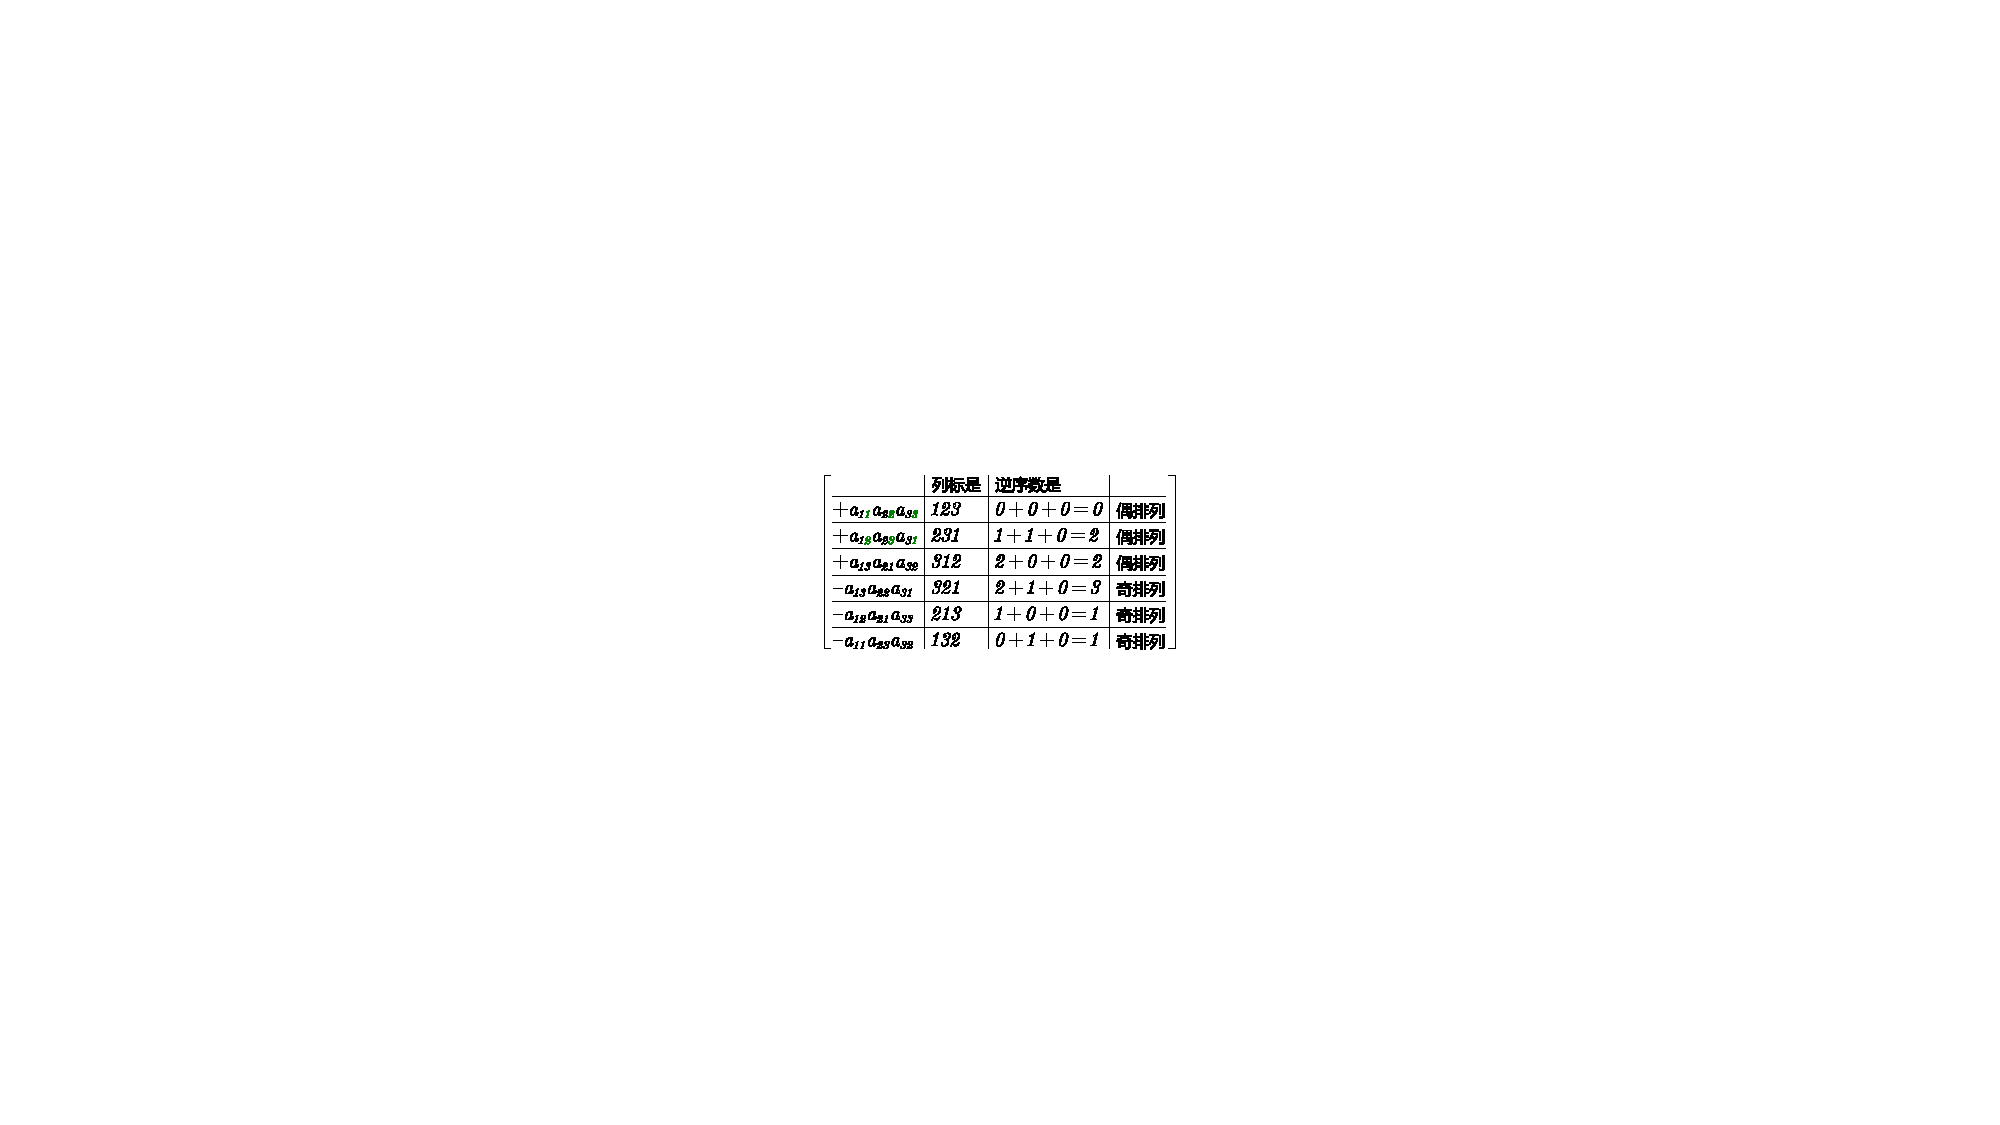
\includegraphics[width=0.5\textwidth]{img/0002.pdf}\\
	
	可以看出: 各项前的正负符号, 是由``列标"的奇偶性(奇排列还是偶排列)决定的 (奇负, 偶正).\\
	- 每一项, 就是从这个行列式的``不同行, 不同列"中, 取出3个元素, 来相乘.\\
	
	上面这个, 即``n阶行列式"的第一种定义方式. 也就是``按行展开".\\
	
	
	\subsection{n 阶行列式 -- 按行展开}
	
	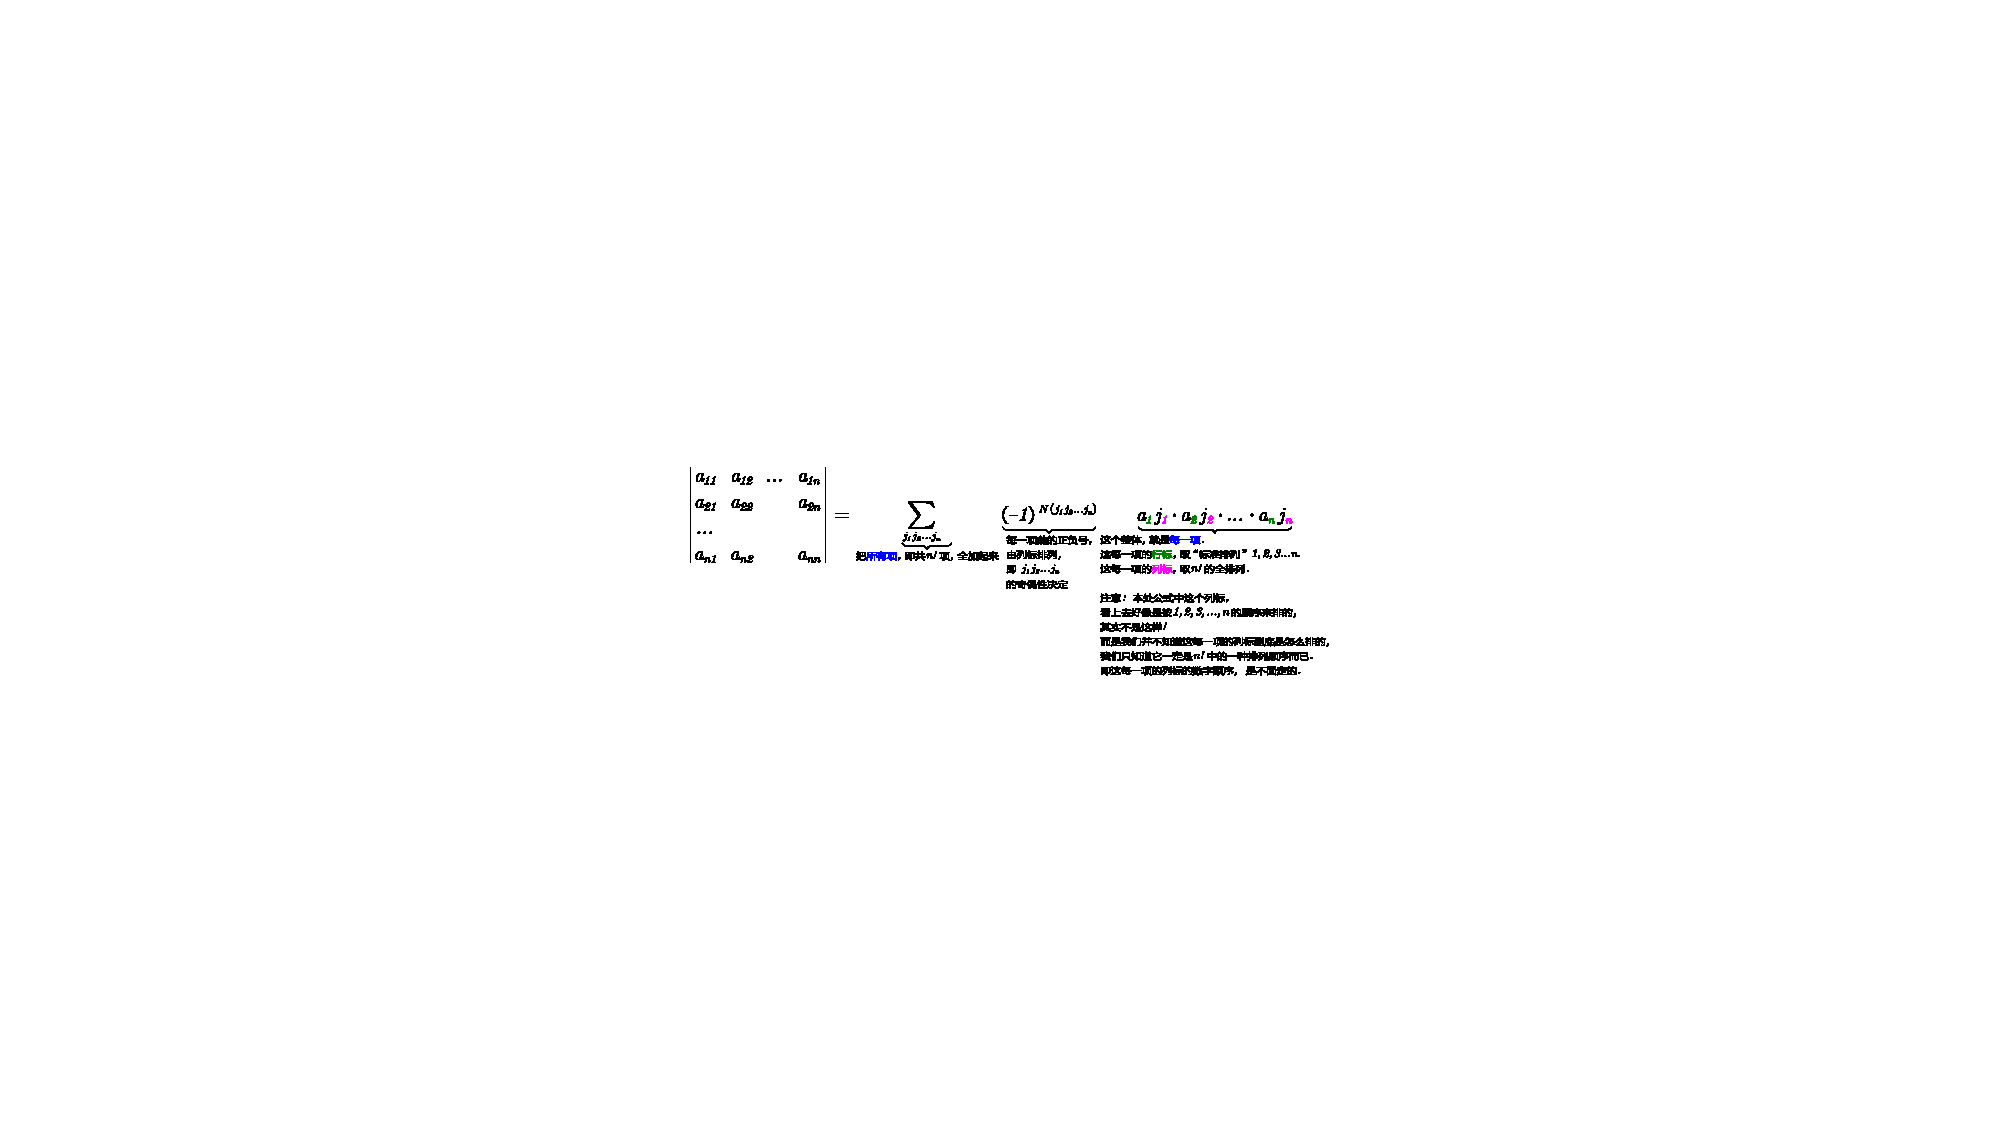
\includegraphics[width=1\textwidth]{img/0003.pdf}\\
	
	n阶行列式的展开, 一共有多少项呢? 共有 n! 项. \\
	
	行列式, 用 D (determinant) 来表示. 写成: $	D=\left| a_{ij} \right|	$
	
	\begin{myEnvSample}
	determinant : n. ( formal ) a thing that decides whether or how sth happens 决定因素;决定条件
	\end{myEnvSample}

	只有一个元素的行列式, 就等于该元素本身, 即:	$	\left| a_{11} \right|=a_{11}	$\\
	|8|=8\\
	|-1|=-1\\
	
	\begin{myEnvSample}
$
\left| \begin{matrix}
	&		2&		&		\\
	&		&		3&		\\
	&		&		&		4\\
	1&		&		&		\\
\end{matrix} \right|=\left( -1 \right) ^{N\left( 2341 \right)}\ 2\cdot 3\cdot 4\cdot 1=-24
$
	\end{myEnvSample}
	
	
	
\subsubsection{下三角行列式 =主对角线上元素的乘积}

$
\underset{\text{下三角行列式}}{\underbrace{\left| \begin{matrix}
			a_{11}&		&		&	0	\\
			a_{21}&		a_{22}&		&		\\
			...&		&		...&		\\
			a_{n1}&		...&		...&		a_{nn}\\
		\end{matrix} \right|}}=\underset{\text{即主对角线元素相乘}}{\underbrace{a_{11}\cdot a_{22}\cdot ...\cdot a_{nn}}}
$



\subsubsection{上三角行列式 =主对角线上元素的乘积}

$
\underset{\text{上三角行列式}}{\underbrace{\left| \begin{matrix}
			a_{11}&		...&		&		a_{1n}\\
			&		a_{22}&		&		a_{2n}\\
			&		&		...&		...\\
			0&		&		&		a_{nn}\\
		\end{matrix} \right|}}=\underset{\text{即主对角线元素相乘}}{\underbrace{a_{11}\cdot a_{22}\cdot ...\cdot a_{nn}}}
$


\subsubsection{对角形行列式 =主对角线上元素的乘积}
$
\underset{\text{对角形行列式}}{\underbrace{\left| \begin{matrix}
			a_{11}&		&		&		0\\
			&		a_{22}&		&		\\
			&		&		...&		\\
			0&		&		&		a_{nn}\\
		\end{matrix} \right|}}=\underset{\text{即主对角线元素相乘}}{\underbrace{a_{11}\cdot a_{22}\cdot ...\cdot a_{nn}}}
$


\subsubsection{伪下三角行列式  $	=\left( -1 \right) ^{\frac{n\left( n-1 \right)}{2}}a_{1,n}\cdot a_{2,n-1}\cdot a_{n,1}	$}

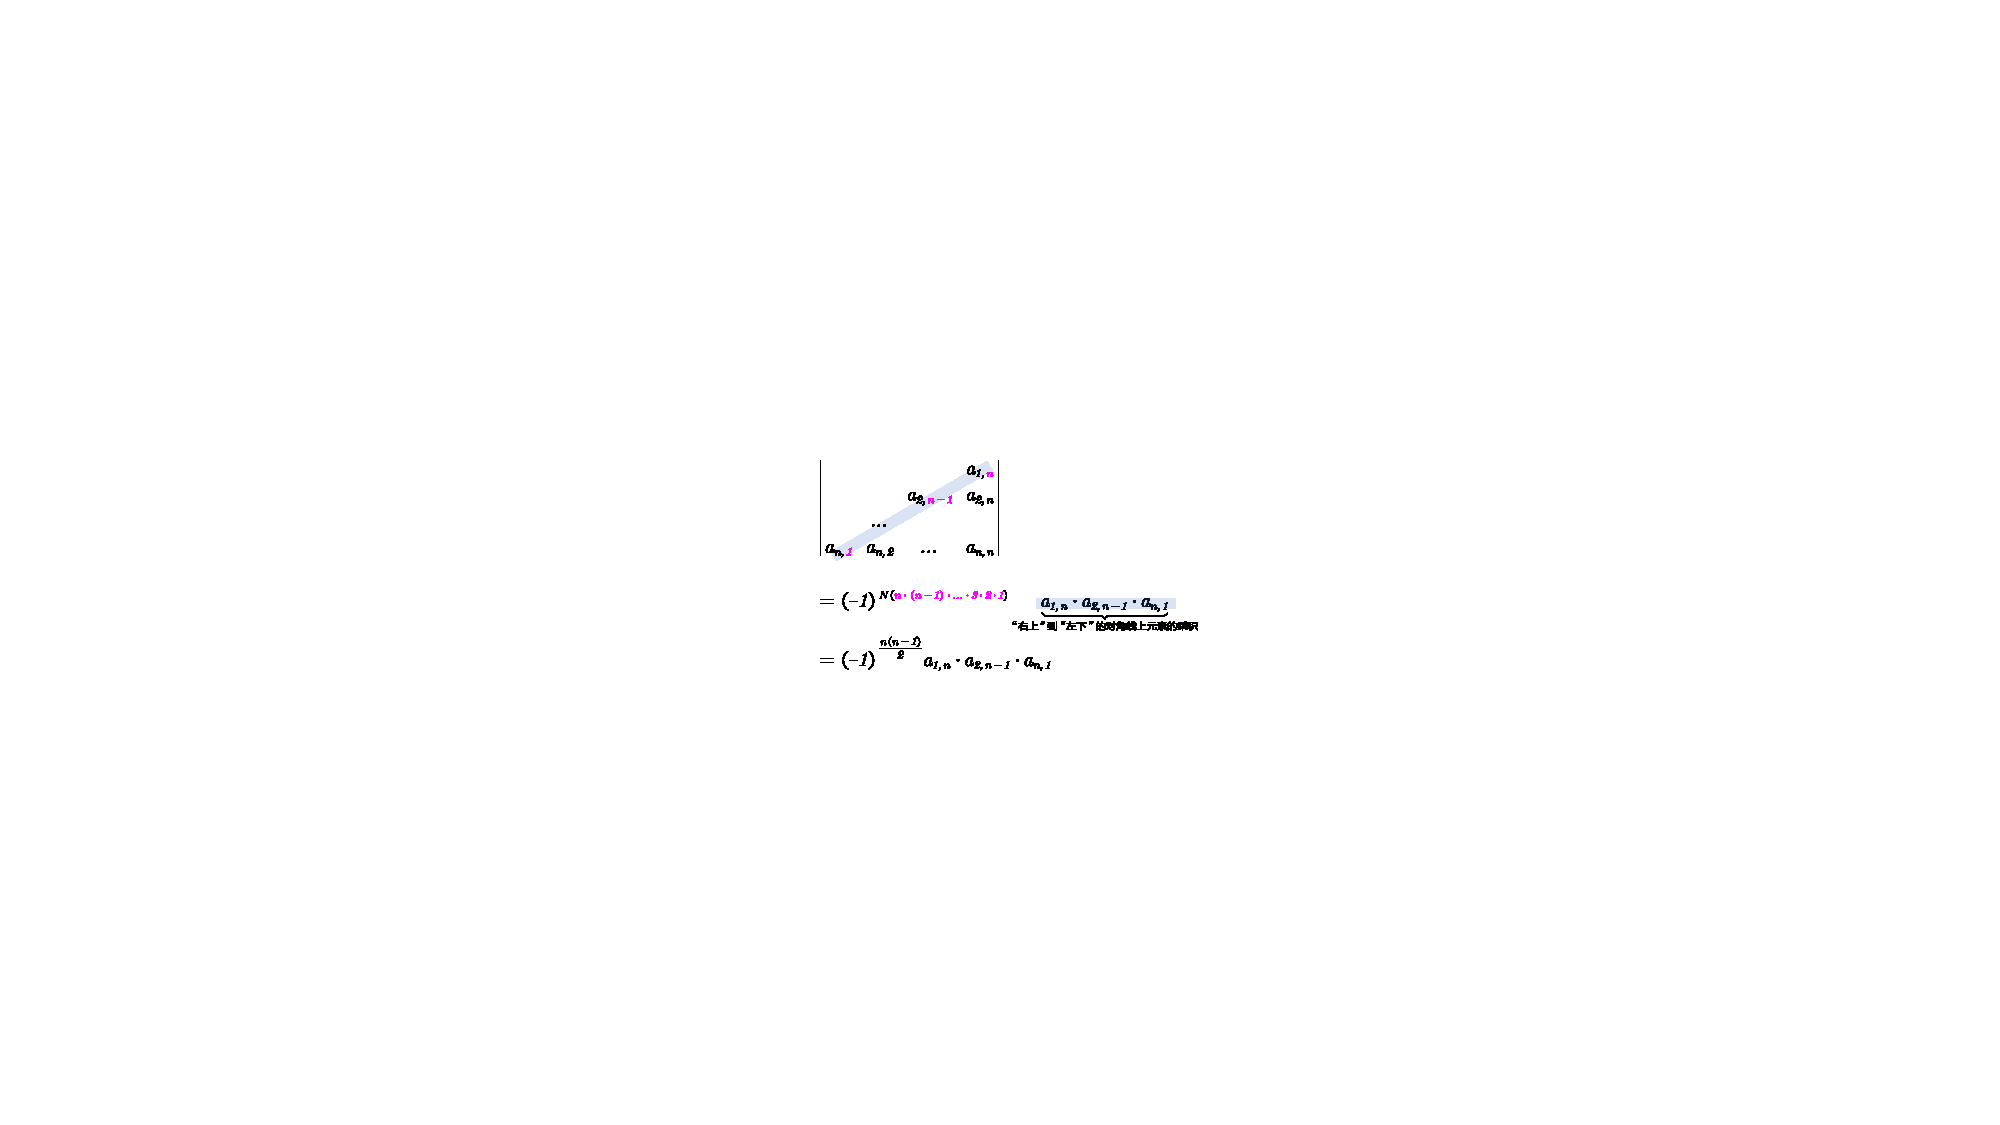
\includegraphics[width=0.6\textwidth]{img/0004.pdf}\\



\subsubsection{伪上三角行列式 $	=\left( -1 \right) ^{\frac{n\left( n-1 \right)}{2}}a_{1,n}\cdot a_{2,n-1}\cdot a_{n,1}	$}

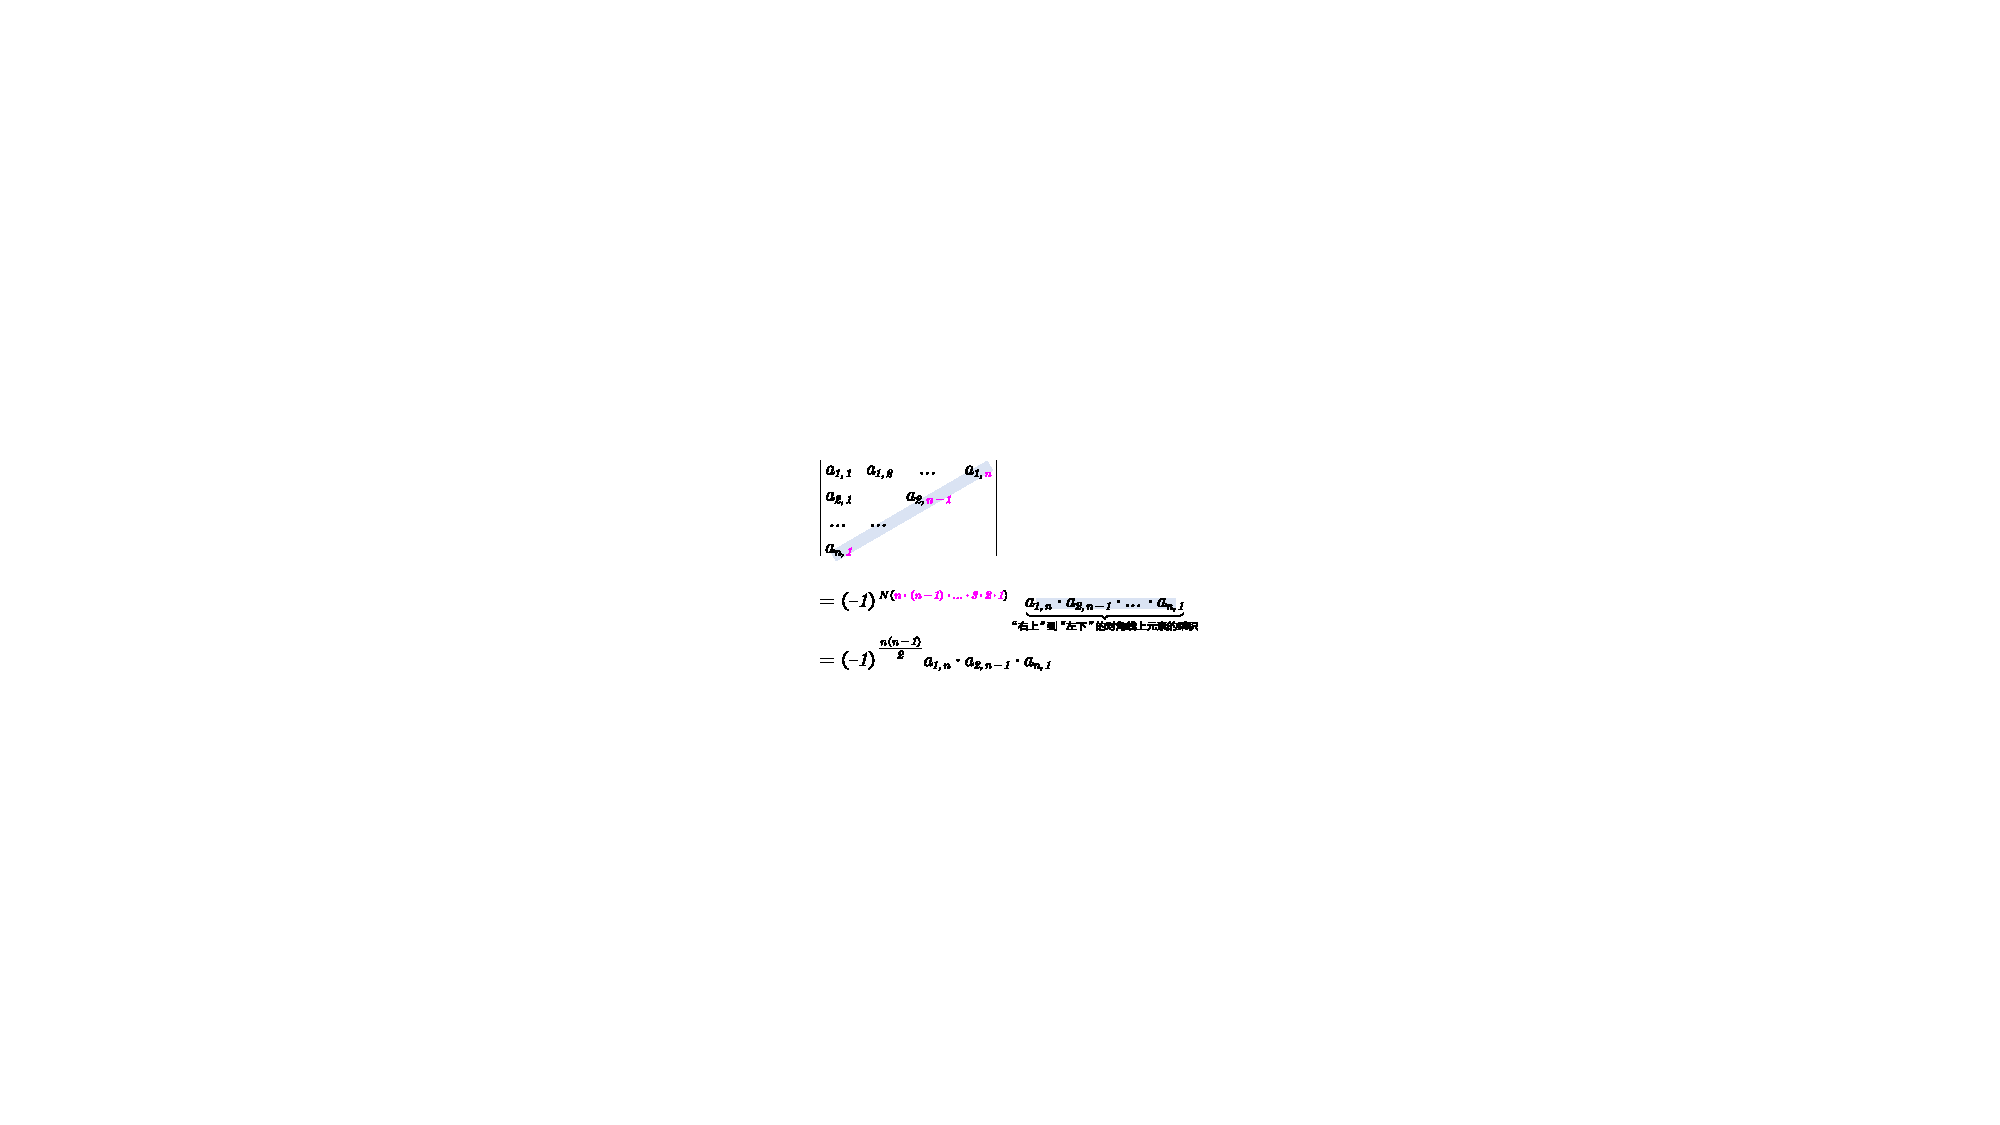
\includegraphics[width=0.6\textwidth]{img/0005.pdf}\\




https://www.bilibili.com/video/BV1aW411Q7x1?p=2&vd_source=52c6cb2c1143f8e222795afbab2ab1b5
31.58
	
	
	
	\section{行列式的性质}
	
	
	\section{行列式按行(列)展开}
	
	
	
	
	--------------------------------
	
	\section{n阶行列式}
	
	
	\section{行列式的性质}
	
	\subsection{性质1: 行列互换, 其值不变. 即$|A|=\left| A^T \right|$}
	
	\subsection{性质2: 某行(列)元素全为零, 则行列式为零}
	
	\subsection{性质3: 两行(列)元素相等, 或对应成比例, 则行列式为零}
	
	\subsection{性质4: 某行(列)元素均是两个元素之和, 则可拆成两个行列式之和}
	
	\subsection{性质5: 两行(列)互换,行列式的值反号}
	
	\subsection{性质6: 某行(列)元素有公因子$k\left( k\ne 0 \right) $, 则k可提到行列式外面去 }
	
	\subsection{性质7: 某行(列)的b, 倍加到另一行(列)上去, 行列式的值不变 }
	
	
	\section{行列式的展开定理}
	
	\subsection{余子式 $M_{ij}$}
	
	\subsection{代数余子式 $	A_{ij}=\left( -1 \right) ^{i+j}M_{ij}$}
	
	\subsection{按某一行(列)展开的展开公式: \\ $|A|=\sum_{i=1}^n{a_{ij}A_{ij}\ \left( j=1,2,...,n \right)}=\sum_{j=1}^n{a_{ij}A_{ij}\ \left( i=1,2,...,n \right)}$	}
	
	
	
	\section{具体型行列式的计算: $a_{ij}$ 已给出}
	
	\subsection{化为``12+1"型行列式}
	
		\subsubsection{主对角线行列式}
		
		\subsubsection{副对角线行列式}
		
		\subsubsection{拉普拉斯展开式}
		
		\subsubsection{范德蒙德行列式}
	
	\subsection{加边法}
	
	\subsection{递推法 (高阶 → 低阶)}
	
		\subsubsection{建立递推公式,即建立$D_n$ 与 $D_{n-1}$ 的关系}
		
		\subsubsection{$D_n$ 与 $D_{n-1}$ 要有完全相同的元素分布规律, 只是$D_{n-1}$比$D_n$低了一阶 }
	
	
	\subsection{数学归纳 (低阶 → 高阶)}
	
		\subsubsection{第一数学归纳法}
		
		\subsubsection{第二数学归纳法}
	
	
	\section{抽象型行列式的计算: $a_{ij}$ 未给出	}
	
		\subsection{用行列式性质}
		
		\subsection{用矩阵知识}
		
			\subsubsection{设 C=AB, A,B为同阶方阵, 则 $|C|=|AB|=|A||B|$}
			
			\subsubsection{设 C=A+B, A,B为同阶方阵, 则 $|C|=|A+B|$,作恒等变形,转化为矩阵乘积的行列式 }
			
			\subsubsection{设A 为n阶方阵, 则 $|A^*|=|A|^{n-1},\ |(A^*)^*|=\left| \left| A \right|^{n-2}A \right|=\left| A \right|^{\left( n-1 \right) ^2}	$}
		
		\subsection{用相似理论}
		
			\subsubsection{$\left| A \right|=\prod_{i=1}^n{\lambda _i}$}
			
			\subsubsection{若A相似于B, 则 |A|=|B|}
	
	
	
\end{document}